\section{EXPERIMENTS} \label{sec:experiments}

In this section we present numerical results of the validation benchmark and
  discuss a proof of concept application in the domain of particle
  accelerators.

\subsection{Optimizer Validation}

\begin{figure}
    \centering
    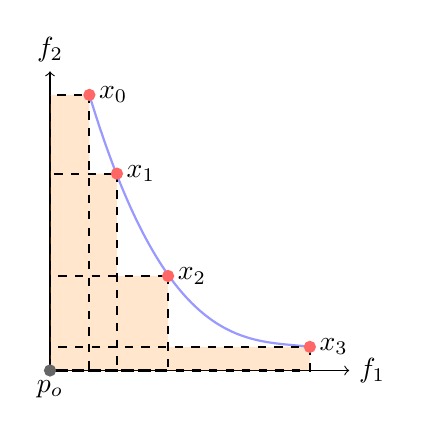
\begin{tikzpicture}[text=black]
      \coordinate (y) at (0,3.8);
\coordinate (x) at (3.8,0);
\draw[<->] (y) node[above] {$f_2$} -- (0,0) --  (x) node[right]
{$f_1$};

\path
  coordinate (start) at (0.5,3.5)
  coordinate (c1) at +(1.5,0.2)
  coordinate (c2) at +(2.5,0.4)
  coordinate (top) at (3.3,0.3);

\draw [thick, blue!40!white] (start) .. controls (c1) and (c2) .. (top);
(start) .. controls (c1) and (c2) .. (top) -- (3.3,0.0);
%\draw [fill, color=blue, draw opacity=0, fill opacity=0.2] (0,0) -- (0.0, 3.5) --
%(start) .. controls (c1) and (c2) .. (top) -- (3.3,0.0);


\draw[fill, color=orange, draw opacity=0, fill opacity=0.2] (0,0) -- (0, 3.5) --
(start) -- (0.5,2.5) -- (0.85, 2.5) -- (0.85, 1.2) -- (1.5, 1.2) -- (1.5, 0.3) -- (top) -- (3.3, 0.0);
\draw[dashed, thick] (start) rectangle (0,0);
\draw[dashed, thick] (top) rectangle (0,0);
\draw[dashed, thick] (0.85,2.5) rectangle (0,0);
\draw[dashed, thick] (1.5,1.2) rectangle (0,0);

\filldraw [red!60!white]
(start) circle (2pt) node[right, black] {$x_0$}
(0.85,2.5) circle (2pt) node[right, black] {$x_1$}
(1.5,1.2) circle (2pt) node[right, black] {$x_2$}
(top) circle (2pt) node[right, black] {$x_3$};

\filldraw [black!60!white]
(0,0) circle (2pt) node[below, black] {$p_o$};


    \end{tikzpicture}
  \caption{The hypervolume for a two-objective optimization problem
  corresponds to the shaded area formed by the dashed rectangles spanned by
  all points on the Pareto front and an arbitrary selected origin $p_o$.}
  \label{fig:hypervolume}
\end{figure}

To ensure that the optimizer works correctly we solved the benchmark
  problem (\ref{eqn:bench}).
To that end, we use a metric for comparing the quality of a Pareto
  front.
Given a point in the Pareto set, we compute the $m$ dimensional volume (for
  $m$ objectives) of the dominated space, relative a chosen origin.
We visualize this for $2$ objectives in Figure~\ref{fig:hypervolume}.
For further information and details of the implementation see~\cite{whbb:12}.
Figure~\ref{fig:pisa_bench} and the corresponding hypervolume values in
  Table~\ref{tbl:bench_rms_error}.
The reference Pareto front is clearly very well approximated.
It took a total of 1100 function evaluations to perform this computation.
The hypervolume of the reference solution ($0.6575$) for our benchmark was
  computed by sampling the solution provided in~\cite{hbwh:05}.

\begin{figure}
  \centering
    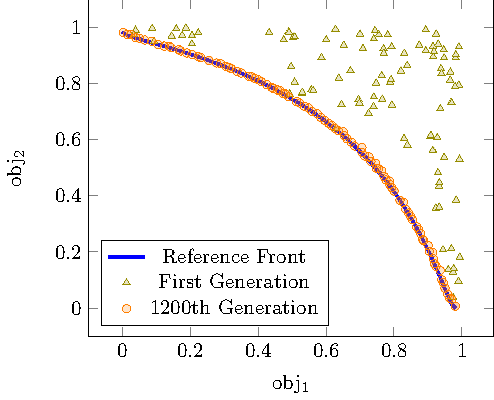
\includegraphics[width=0.7\linewidth]{figures/valid_front}
  \caption{Variator benchmark after $1100$ function evaluations using binary
           crossover and independent gene mutations (each gene mutates with
           probability $p=\frac{1}{2}$) on a population of $100$
           individuals.}
  \label{fig:pisa_bench}
\end{figure}

\begin{table}%[h!]
\begin{center}
  \caption{Convergence of benchmark problem with errors relative to
    hypervolume of sampled reference solution.}
  \label{tbl:bench_rms_error}
  \begin{tabular}{lcc}
    \hline\noalign{\smallskip}
    tot.\ function  & hyper volume & relative error\\
    evaluations    & & \\
    \noalign{\smallskip}\hline\noalign{\smallskip}
    100  &  0.859753 & $3.076 \times 10^{-1}$ \\
    \noalign{\smallskip}\hline\noalign{\smallskip}
    200  &  0.784943 & $1.938 \times 10^{-1}$ \\
    500  &  0.685183 & $4.210 \times 10^{-2}$ \\
    900  &  0.661898 & $6.689 \times 10^{-3}$ \\
    1100 &  0.657615 & $1.749 \times 10^{-4}$ \\
    \noalign{\smallskip}\hline
  \end{tabular}
\end{center}
\end{table}

From Table~\ref{tbl:bench_rms_error} we deduce that we achieved satisfactory
  convergence to the sampled reference Pareto front after 1000 (plus the
  additional 100 evaluations for the initial population) function evaluations.


\subsection{Ferrario Matching Point}\label{ferrario}

As a verification and proof of concept we reproduce the Ferrario
  matching point discovered by Ferrario \textit{et~al.}~\cite{fcpr:00},
  by formulating the problem as a  multi-objective optimization problem.
Using the low-dimensional and fast nature of their new simulation code
  Homdyn~\cite{homdyn}, an extensive beam dynamics study was conducted.

One of the results of the study presented in \cite{fcpr:00} was the discovery
  of a novel working point.
The authors noticed that the second emittance minimum can profit from the
  additional emittance compensation in the accelerating traveling wave
  structure ensuring that the second emittance minimum occurs at a higher
  energy.
This property is attained if the beam emittance has a maximum and the root
  mean square (rms) beam size has a minimum at the entrance of the first
  accelerating traveling wave structure.
This behavior is illustrated in Figure~\ref{fig:fer_match}.

\begin{figure}
  \centering
  
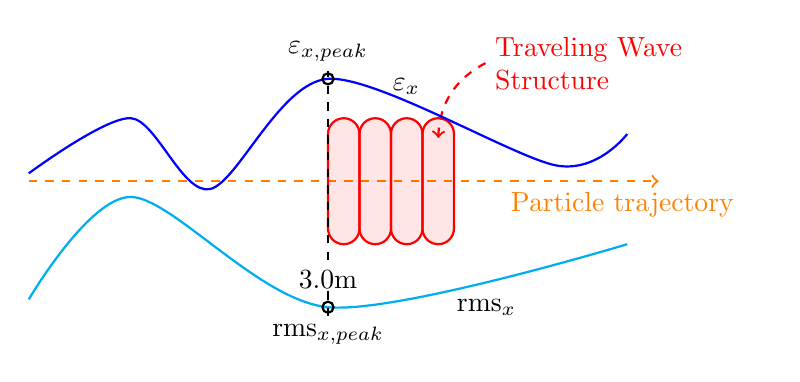
\begin{tikzpicture}

  \draw[dashed, thick, color=orange] (1.2,2.0) edge[->] (9.2,2);
  \node[orange, right, text width=3.2cm] at (7.2, 1.7) {Particle trajectory};

  %\draw[thick] (1.2,2.5) edge (9,2.5);
  %\draw[thick] (1.2,1.5) edge (9,1.5);
  %\node[above] at (1.0, 1.45) {Beam pipe};

  \draw[thick,color=red, fill=red, fill opacity=0.1, rounded corners=2mm] (5.0,1.2)
      rectangle (5.4,2.8);
  \draw[thick, dashed] (5.0,1.0) edge (5.0,3.4) node[below] {$3.0$m};
  \draw[thick,color=red, fill=red, fill opacity=0.1, rounded corners=2mm] (5.4,1.2)
      rectangle (5.8,2.8);
  \draw[thick,color=red, fill=red, fill opacity=0.1, rounded corners=2mm] (5.8,1.2)
      rectangle (6.2,2.8);
  \draw[thick,color=red, fill=red, fill opacity=0.1, rounded corners=2mm] (6.2,1.2)
      rectangle (6.6,2.8);
  \node[right, red, text width=2.8cm] at (7.0, 3.5) {Traveling Wave Structure};
  \draw[dashed, thick, color=red, bend right] (7.0,3.5) edge[->] (6.4,2.55);

  \draw[thick, cyan] plot [smooth, tension=0.5] coordinates {
      (1.2,0.5)
      (2.5,1.8)
      (5.0,0.4)
      (8.8,1.2)};
  \draw[thick, dashed] (5.0,0.6) edge (5.0,0.2);
  \draw[thick] (5.0,0.4) circle (2pt);
  \node[very thick, right] at (6.5, 0.4) {rms$_x$};
  \node[below] at (5.0, 0.3) {rms$_{x\text{, peak}}$};

  \draw[thick, blue] plot [smooth, tension=0.5] coordinates {
      (1.2,2.1)
      (2.5,2.8)
      (3.5,1.9)
      (5.0,3.3)
      (7.9,2.2)
      (8.8,2.6)};
  \draw[thick] (5.0,3.3) circle (2pt);
  \node[right] at (5.7, 3.2) {$\varepsilon_x$};
  \node[above] at (5.0, 3.4) {$\varepsilon_{x\text{, peak}}$};

\end{tikzpicture}

  \caption{Illustration of the Ferrario matching criteria: beam emittance
  attains a maximum and rms beam size a minimum at the entrance to the first
  accelerating traveling wave structure.}
  \label{fig:fer_match}
\end{figure}

By artificially reproducing this working point as the solution of a
  multi-objective optimization problem given in equations
  (\ref{eq:swissfel:p1}) to (\ref{eq:swissfel:lastdvar}),
  we demonstrate the automation of discovering optimal beam dynamics behaviors
  given a set of desired objectives.

\begin{align}
\text{min}  \quad & \left[ \Delta \text{rms}_{x,\text{peak}} = \vert 3.0 -
\text{rms}_{x,\text{peak}} \vert, \right. \label{eq:swissfel:p1}\\
                & \Delta \varepsilon_{x,\text{peak}}  = \vert 3.0 -
                \varepsilon_{x,\text{peak}} \vert, \label{eq:swissfel:p2}\\
                & \left. \vert \text{rms}_{x, \text{peak\_pos}} -
                \varepsilon_{x,\text{peak\_pos}} \vert
                \label{eq:swissfel:p3} \right]^T\\
\text{subject to} \quad & q = 200 \left[\text{pC}\right] \label{eq:swissfel:firstconstr}\\
          \quad & \text{Volt}_{\text{RF}} = 100 \left[\text{MV/m}\right] \label{eq:swissfel:lastconstr}\\
          \quad & \sigma_{L} \leq \sigma_x = \sigma_y \leq \sigma_{U} \label{eq:swissfel:firstdvar}\\
          \quad & \text{KS}_{L} \leq \text{KS}_{\text{RF}} \leq \text{KS}_{U} \label{eq:swissfel:seconddvar}\\
          \quad & \text{LAG}_{L} \leq \text{LAG}_{\text{RF}} \leq \text{LAG}_{U} \\
          \quad & \Delta z_{L\text{KS}} \leq \Delta z_{\text{KS}} \leq \Delta z_{U\text{KS}} \label{eq:swissfel:lastdvar}
\end{align}

The first two objectives minimize the distance from the position of the current
  minimum peak to the expected peak location at $3.0$\,m for transverse bunch
  size (beam waist) and emittance (see Figure~\ref{fig:fer_match}).
The third objective (\ref{eq:swissfel:p3}) adds a condition preferring
  solutions that have their emittance and rms peak locations at the same
  $s$-coordinate.
Equations (\ref{eq:swissfel:firstconstr}) and (\ref{eq:swissfel:firstdvar})
  define constraints for initial conditions for the simulation: charge,
  gun voltage and laser spot size.
Design variables given in (\ref{eq:swissfel:seconddvar}) to
  (\ref{eq:swissfel:lastdvar}) correspond to field strengths of the
  first focusing magnet, its displacement, and the phase of the gun.

In order to compute the peaks, we employed an additional Python script.
This script was called in the \textsc{OPAL}~input file, after the simulation
  finished using the \texttt{SYSTEM} functionality.
Once the peaks (in a given range) were located, the two objectives
  (\ref{eq:swissfel:p1}) and (\ref{eq:swissfel:p2}) were computed and their
  values written into corresponding files.
The custom \texttt{fromFile} functor allows us to access the values stored in
  the peak finder Python script result files
%
%\vspace{0.2cm}

\begin{flushleft}
\begin{Verbatim}[fontsize=\scriptsize]
rmsx:  OBJECTIVE, EXPR="statVariableAt("rms_x-err.dat", "var")";
emitx: OBJECTIVE, EXPR="statVariableAt("emit_x-err.dat", "var")";
match: OBJECTIVE, EXPR="fabs(statVariableAt("emit_x-peak.dat", "var") -
statVariableAt("rms_x-peak.dat", "var"))";
\end{Verbatim}
\end{flushleft}
\vspace{0.2cm}

\noindent
The design variables and the assembly of the multi-objective optimization problem
  can be included in the \textsc{OPAL}~input file as shown below:
%\vspace{0.2cm}

\begin{flushleft}
\begin{Verbatim}[fontsize=\scriptsize]
d1: DVAR, VARIABLE="SIGX", LOWERBOUND="0.00025", UPPERBOUND="0.00029";
d2: DVAR, VARIABLE="FIND1_MSOL10_i", LOWERBOUND="110", UPPERBOUND="120";
d3: DVAR, VARIABLE="D_LAG_RGUN", LOWERBOUND="-0.1", UPPERBOUND="0.1";
d4: DVAR, VARIABLE="D_SOLPOS", LOWERBOUND="-0.05", UPPERBOUND="0.05";

objs:    OBJECTIVES = (rmsx, emitx);
dvars:   DVARS = (d1, d2, d3, d4);
constrs: CONSTRAINTS = ();
opt:     OPTIMIZE, OBJECTIVES=objs, DVARS=dvars,
CONSTRAINTS=constrs;
\end{Verbatim}
\end{flushleft}
\vspace{0.2cm}

%All numerical experiments in this sections were executed on the
%  \textsc{Felsim} cluster at PSI\@.
%The \textsc{Felsim} cluster consists of 8 dual quad-core Intel Xeon
%  processors at 3.0 GHz and has $2$ GB memory per core with a total of 128
%  cores.
%The nodes are connected via Infiniband network with a total bandwidth of 16
%  GB/s.

The envelope-tracker, mentioned in the previous section, was used to evaluate
  the forward problems.
We performed a beam convergence study in order to tune the simulation input
  parameters to achieve the best trade-off between simulation accuracy and
  time to solution.
These parameters include the number of slices (\texttt{NSLICE}) used in the
  envelope-tracker simulations, simulation timestep (\texttt{DT}) and gun
  timestep (\texttt{DTGUN}).

Before the simulation can be executed a number of initial beam optics
  parameters have to be defined in an input file.
Table~\ref{tbl:et_params} shows the values of these parameters for the
  envelope-tracker.
All simulations were performed up to 12.5~m of the
  \textsc{SwissFEL} 250 MeV injector~\cite{pedr:10} beam line, with
  energies reaching  up to 120 MeV.

\begin{figure}%[h!]
  \centering
  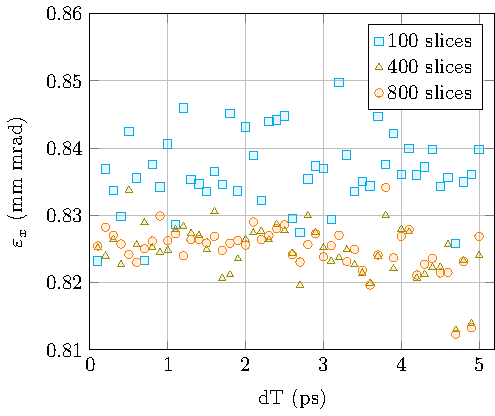
\includegraphics[width=0.8\linewidth]{Report/dt_scan}
  \caption{Envelope-tracker with different number of slices and simulation
    time steps.}
  \label{fig:et-dt}
\end{figure}

\begin{table}
  \begin{center}
    \caption{Initial conditions for the envelope tracker.}
    \label{tbl:et_params}
    \begin{tabular}{ll}
      \hline\noalign{\smallskip}
      name & initial value \\
      \noalign{\smallskip}\hline\noalign{\smallskip}
        Gun voltage       & $100$ MV\\
        %Solenoid current & $110.541$ A\\
        %Laser spot size  & $290 \times 10^{-6}$ m in x and y\\
        Bunch charge      & $200$ pC\\
        %DT$_{Gun}$        & $0.06$ ps\\
        DT$_{\text{Beamline}}$  & $1.5$ ps\\
        Number of slices  & $400$ \\
      \noalign{\smallskip}\hline
    \end{tabular}
  \end{center}
\end{table}

The parameter that affects the performance most is the number of slices.
We scanned the range from $100$ to $1000$ slices to determine the minimal
  number of slices required for stable results using various timesteps.
The results (for 100, 400 and 800 slices) of this scan are shown in
  Figure~\ref{fig:et-dt}.
Using this data we settled for $400$ slices -- increasing the slice number
  only minimally improves convergence of the results, therefore using more
  slices is inefficient.


%\begin{figure}
   %\centering
     %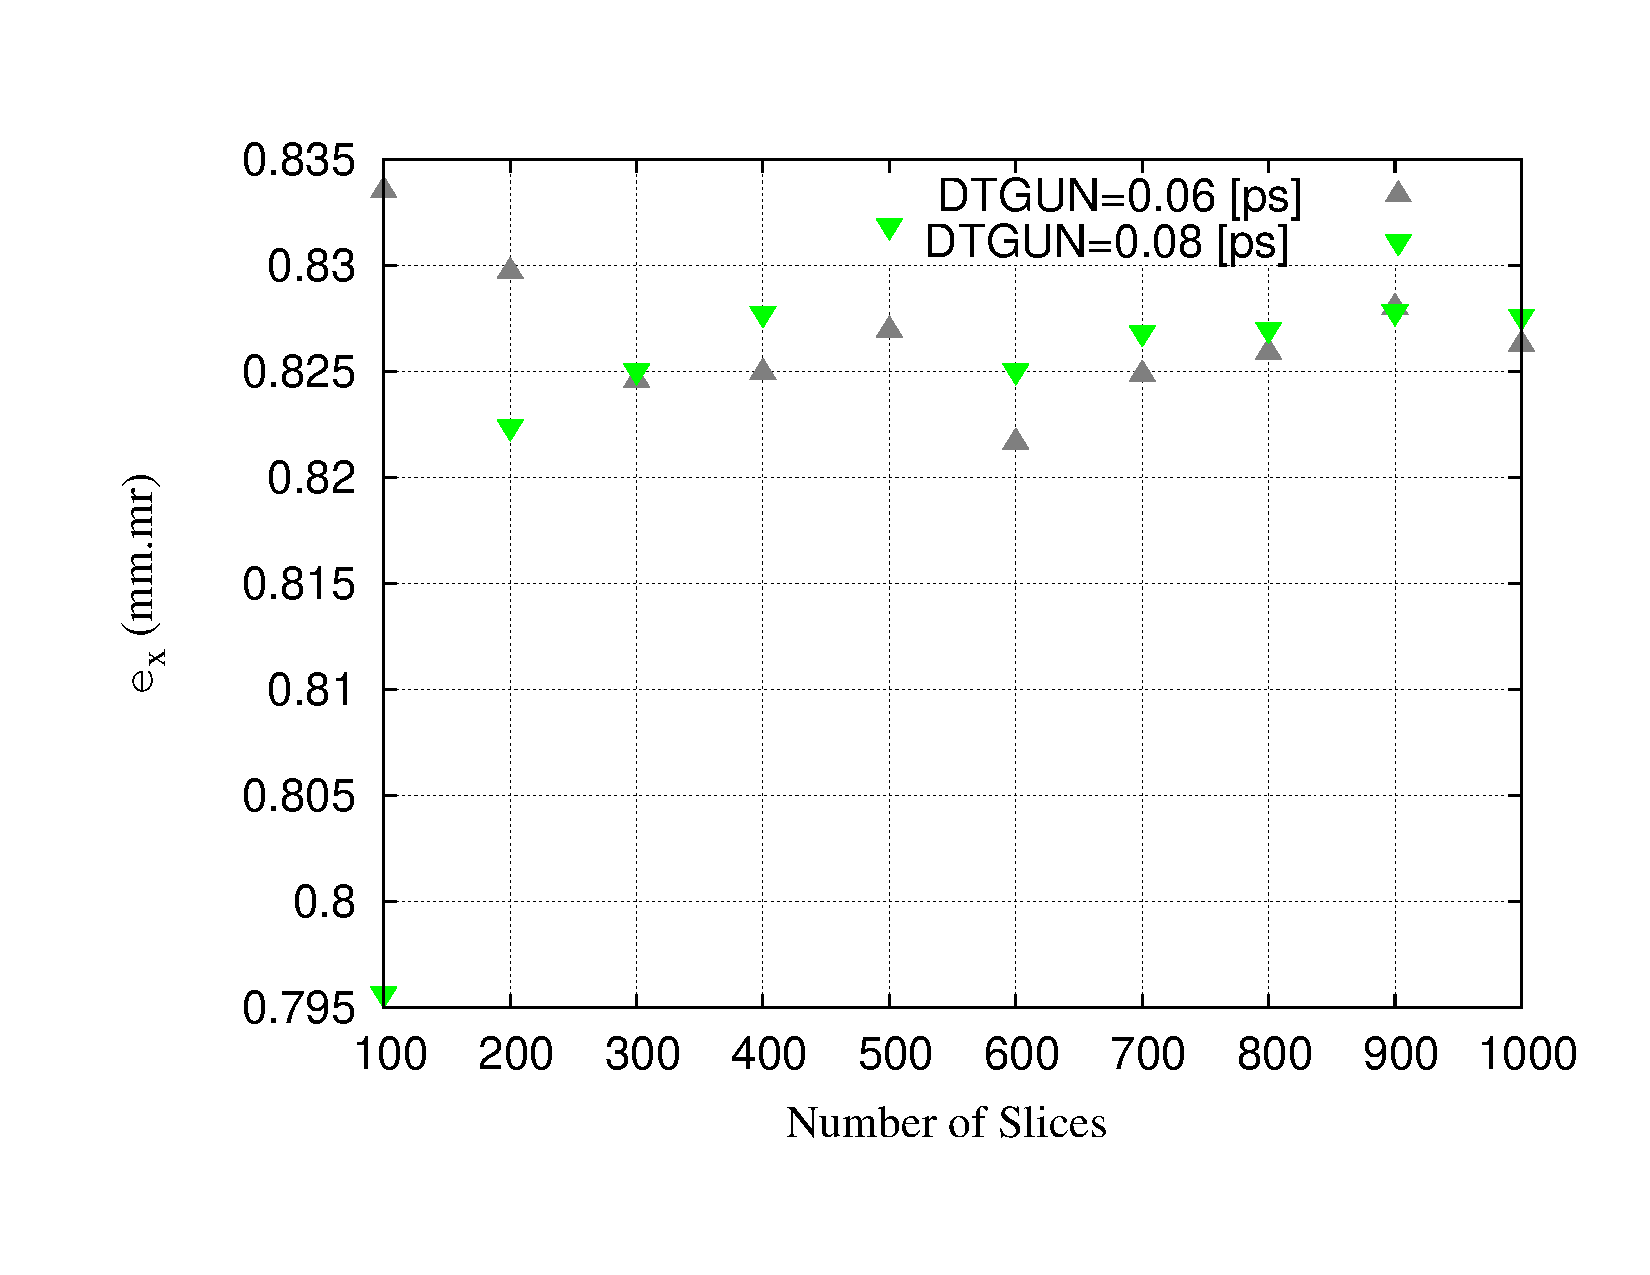
\includegraphics[angle=0,width=0.8\linewidth]{Report/sliceNew}
   %\caption{Scan of the envelope-tracker slice number showing its influence
            %on the exit emittance values.}
   %\label{fig:scan_slices}
%\end{figure}

In a next step the influence of different time steps was examined.
To that end a series of optimization runs with 100, 400 and 800 slices and
  varying timestep was performed.
%Figures \ref{fig:pareto_front_1} and \ref{fig:pareto_front_21} show two Pareto
Figure~\ref{fig:pareto_front_21} shows the Pareto fronts for 400 slices
  respectively using different timesteps.
As expected, increasing the number of slices while lowering the timestep
  produces more detailed results.

%\begin{figure}
  %\centering
    %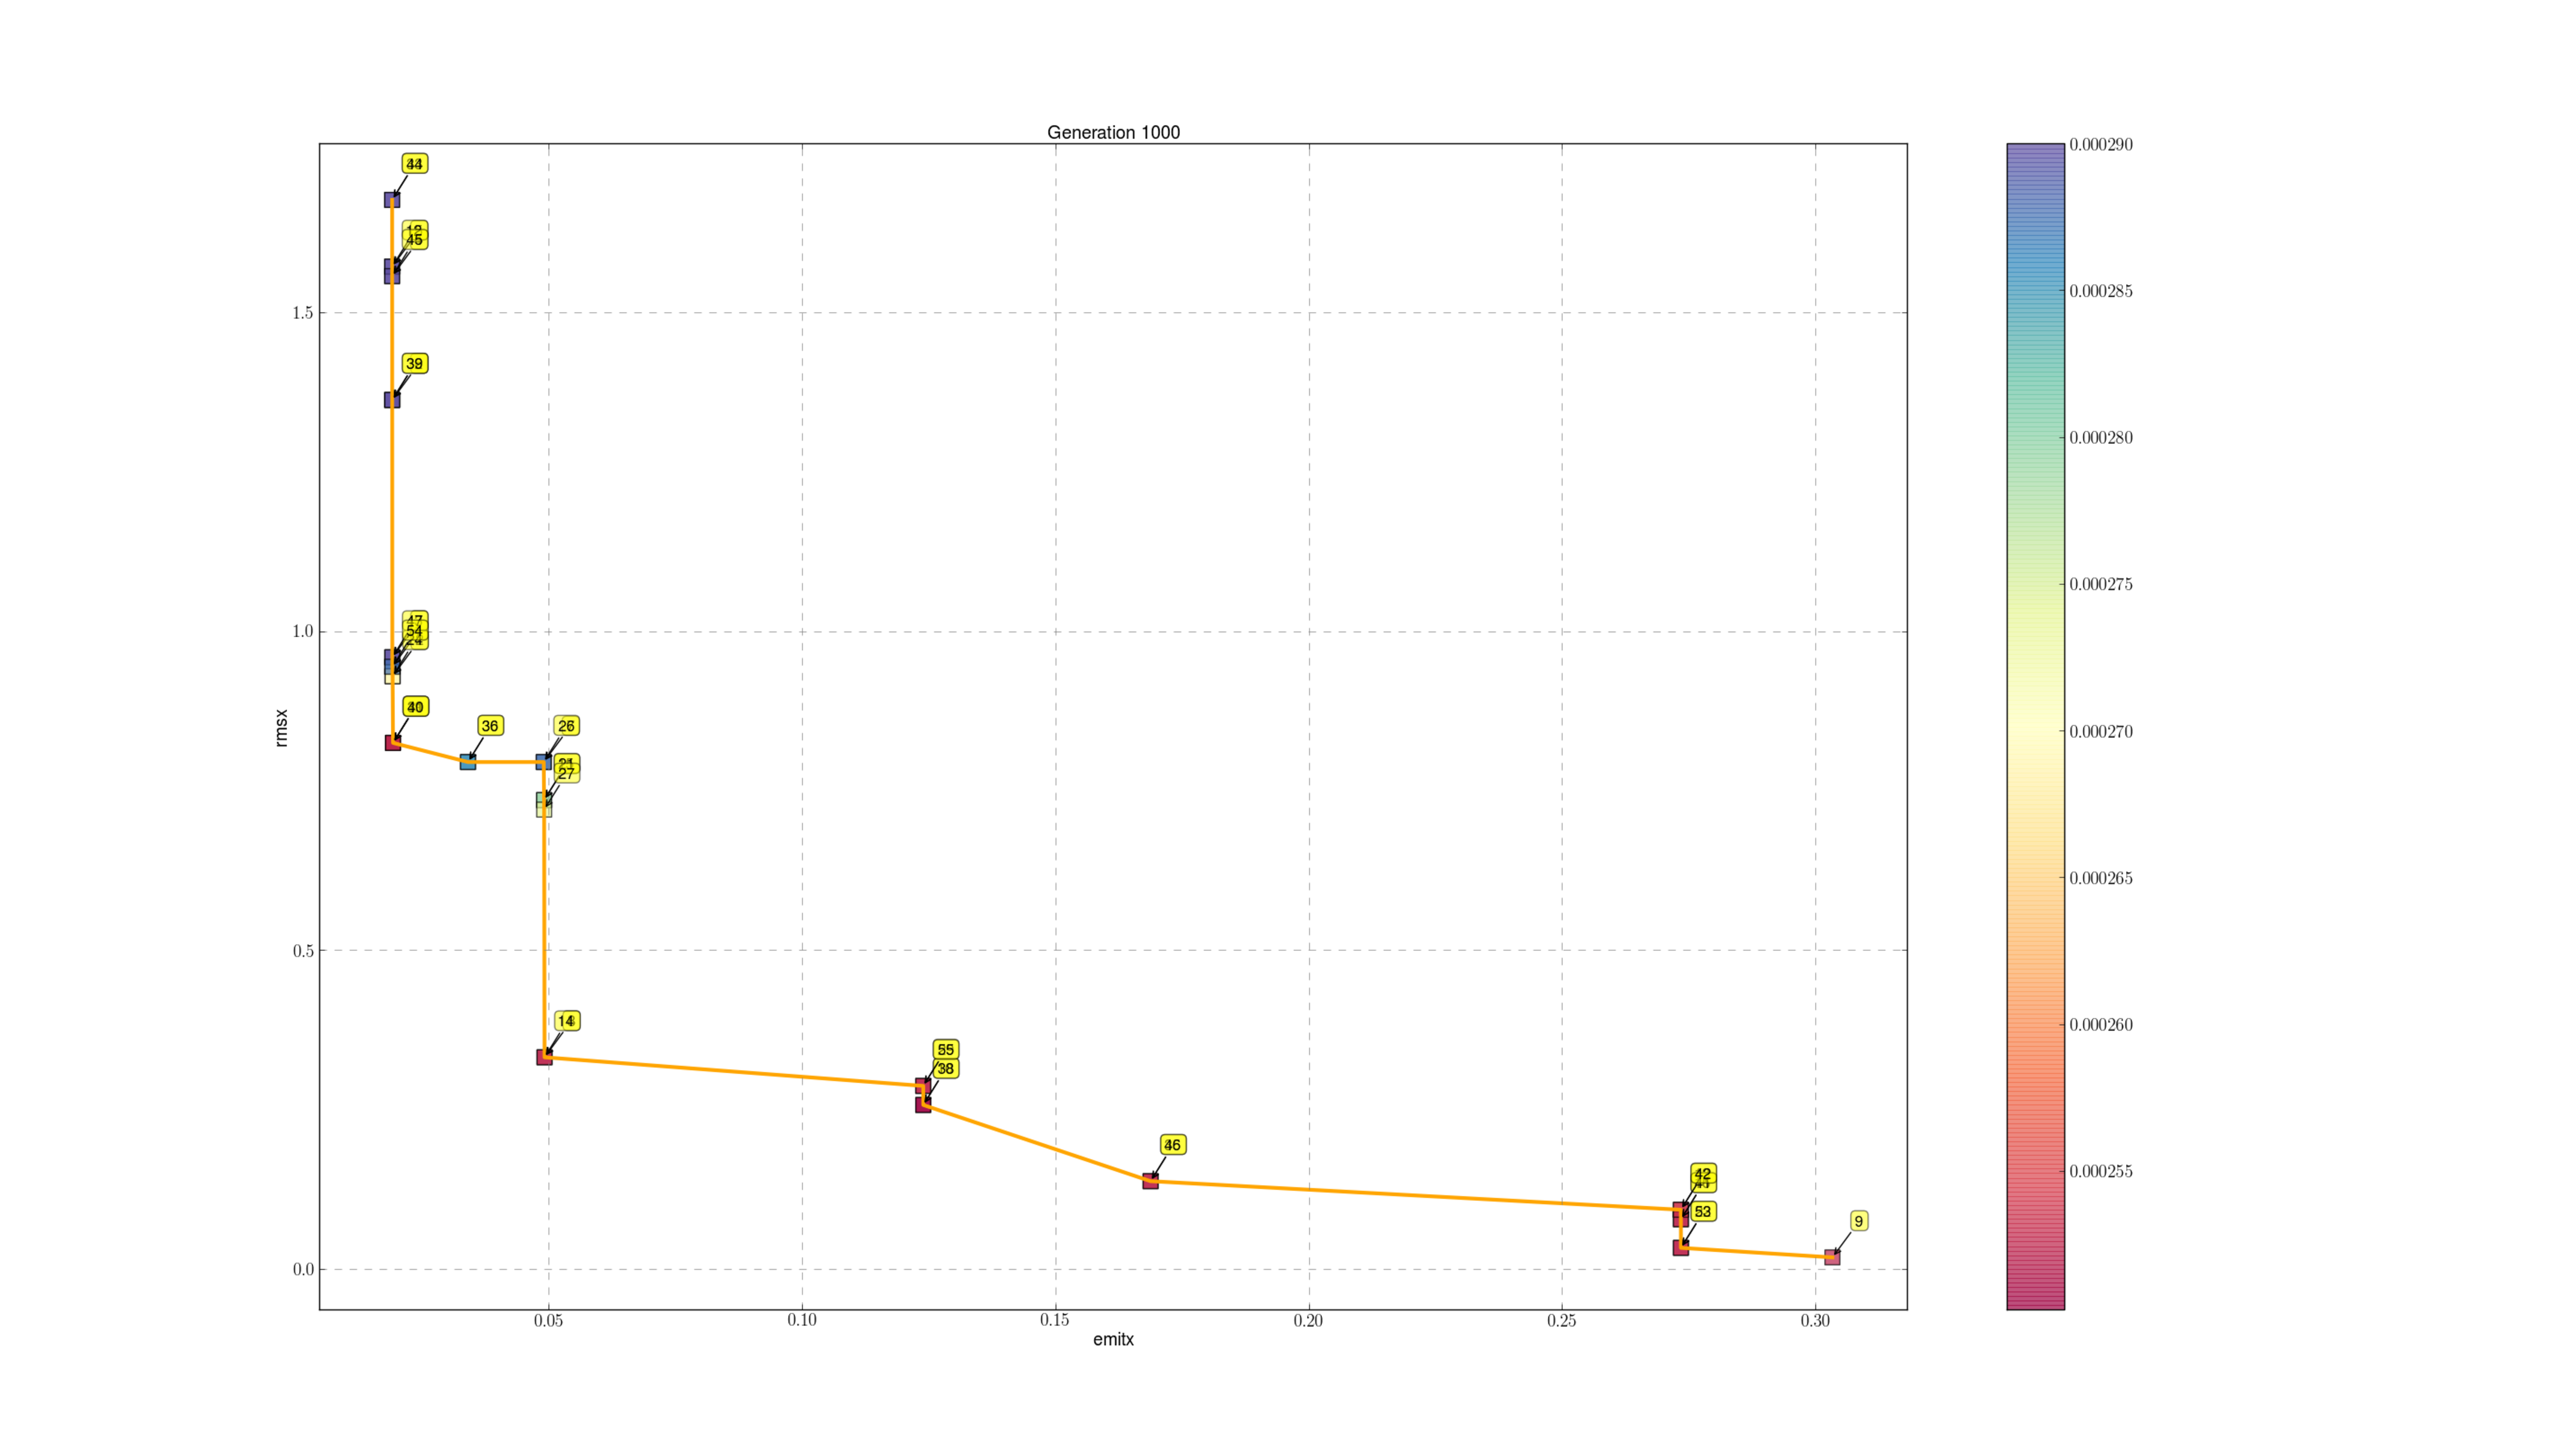
\includegraphics[width=0.9\linewidth]{Report/Run1slices100a}
  %\caption{Pareto Front for the $1000$th generation with $40$ individuals
    %using 100 slices, a simulation timestep of 5 ps and a gun timestep of 0.1
    %ps.}
  %\label{fig:pareto_front_1}
%\end{figure}

\begin{figure}%[h!]
  \centering
    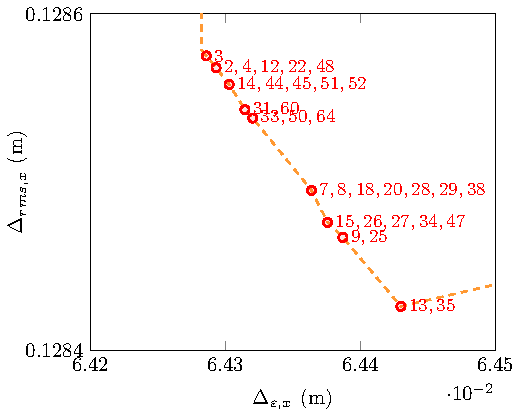
\includegraphics[width=0.8\linewidth]{Report/front_plot}
  \caption{Pareto front for the $1000$th generation with $40$ individuals
    using 400 slices (interesting region magnified), a simulation timestep
    of 1.5 ps.
    The individual 3 was selected for further investigations.}
  \label{fig:pareto_front_21}
\end{figure}


\subsubsection{Optimization Results}

Each of the $40$ points on the Pareto front, shown in
  Figure~\ref{fig:pareto_front_21}, represents an optimal solution, where
  emittance and beam size values are compromised to achieve the best agreement
  with the Ferrario matching point.
We selected individual $3$ based on a comparison of the emittance and beam size
  characteristics of all solutions and by retaining the feasibility of the
  beam line optics parameters.
The design variables, emittance and beam size of the selected solution are
  shown in Table~\ref{tbl:des_vars} and Figure~\ref{fig:rmsemit}.
With the multi-objective optimization framework we attain the same working
  point as reported in~\cite{pedr:10}.

\begin{table}
  \begin{center}
    \caption{The design variables for individual $3$.}
    \label{tbl:des_vars}
    \begin{tabular}{ll}
      \hline\noalign{\smallskip}
      name & value \\
      \noalign{\smallskip}\hline\noalign{\smallskip}
        $\sigma_{x}$          & $0.262$ mm \\
        Solenoid displacement & $28.8467$ mm \\
        Gun voltage lag       & $0.0159067$ MV\\
        Solenoid current      & $111.426$ A \\
      \noalign{\smallskip}\hline
    \end{tabular}
  \end{center}
\end{table}

\begin{figure}%[h!]
  \centering
  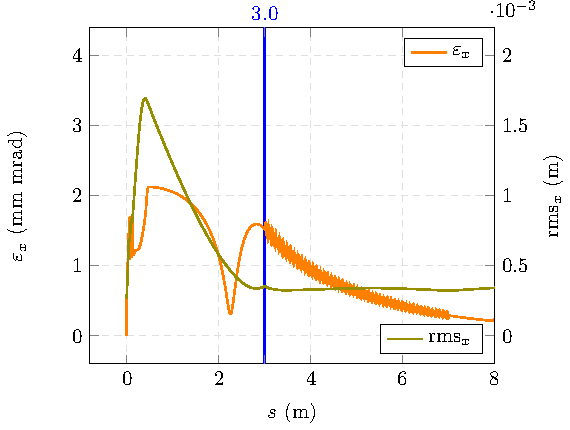
\includegraphics[width=0.8\linewidth]{Report/iff_plot_emrms}
  \caption{Beam size and emittance of individual $3$.}
  \label{fig:rmsemit}
\end{figure}

Using the input parameters of the selected solution, we performed a stability
  analysis by varying the slice number and the time step for both the gun and
  the beam line.
Figure~\ref{fig:et-dt} shows that the exit emittance stabilizes for 400
  slices and various time steps.
No difference between $800$ and $400$ slices is visible as their minimum
  maximum extension seems to be in the same range of $0.024$ mm~mrad.

For validation purposes we compared the results of the envelope-tracker using
  the analytical space charge model with the \textsc{OPAL-t} 3D macro particle
  tracker.
The benchmark was run on the first 12.5 meters of the \textsc{SwissFEL} 250
  MeV injector.
The results for both rms beam size and emittance are shown in
  Figure~\ref{fig:et-vs-tt}.
A good agreement between the two codes can be observed.
The difference of the larger emittance along the solenoids in case of 3D
  tracker that is not seen by the envelope-tracker is due to the different
  definition of the particle momenta (canonical vs.~mechanical).
Both trackers agree within acceptable limits \cite{chao:99}.

\begin{figure}
  \centering
  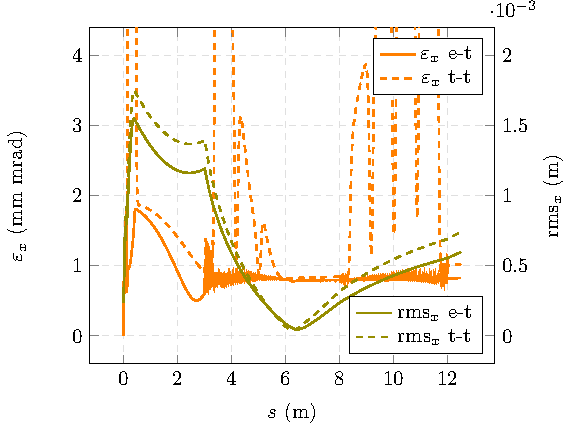
\includegraphics[width=0.9\linewidth]{Report/iff_plot_emrms_ettt}
  \caption{Comparison 3D-tracker versus envelope-tracker in case for rms$_{x}$
    and $\varepsilon_{x}$.}
  \label{fig:et-vs-tt}
\end{figure}

%\subsection{IW2: Inverse Problem}

%In order to find cross correlations we try to solve the inverse problem
  %(15) -- (23)
%%
%\begin{align}
  %\text{min}  \quad & \sqrt{\frac{1}{N} \sum \left( \text{rmx}_{x,s} -
                      %\text{m}_{x,s} \right)^2 } \text{,}\\
              %\quad & \sqrt{\frac{1}{N} \sum \left( \text{rmx}_{y,s} -
                      %\text{m}_{y,s} \right)^2 } \text{,}\\
              %\quad & \sqrt{\frac{1}{N} \sum \left( \text{rmx}_{z,s} -
                      %\text{m}_{z,s} \right)^2 } \\
  %\text{s.t.} \quad & -0.95 \leq \text{R52} \leq -0.65 \label{eq:iw2:fistdvar}\\
              %\quad & -0.90 \leq \text{R61} \leq -0.50 \\
              %\quad & 0.0   \leq \text{R62} \leq 0.20 \\
              %\quad & 0.25 \leq \text{CORR}_x \leq 0.65 \\
              %\quad & 0.55 \leq \text{CORR}_y \leq 0.95 \\
              %\quad & 0.10 \leq \text{CORR}_z \leq 0.50 \label{eq:iw2:lastdvar} \text{.}
%\end{align}
%%
%We try to match the beam to measurements from the real machine by minimizing
  %the sum of $N$ squared measurement ($m_{d,s}$ at a given position
  %$s$) errors for rmx beam size in each dimensions.
%The design variables (\ref{eq:iw2:fistdvar}) - (\ref{eq:iw2:lastdvar}) define
  %the correlation matrix used when generating particles, e.g., R51, R52, R61,
  %R62 describe limits of correlations between planes.
%The initial Binomial distribution (with $m = ?$) has the form
%%
%\begin{equation*}
  %\frac{1}{2\pi\sigma_x\sigma_y}exp(-\frac{x^2}{2\sigma_x^2}
  %-\frac{y^2}{2\sigma_y^2})
  %\text{.}
%\end{equation*}
%%

%Since these correlations cannot be measured we get the real values by solving
  %the inverse problem mentioned above.

%Currently we run the simulations on a low resolution space charge grid ($8
  %\times 8 \times 8$) as a proof of concept.
%In a next step a simple Python script would be applied to iteratively rerun
  %the optimizer with increasing space-charge resolution when the limits of the
  %design variables are narrow enough (iteratively diminishing search space).
%\subsection{IW2: Inverse Problem}

%In order to find cross correlations we try to solve the inverse problem
  %(15) -- (23)
%%
%\begin{align}
  %\text{min}  \quad & \sqrt{\frac{1}{N} \sum \left( \text{rmx}_{x,s} -
                      %\text{m}_{x,s} \right)^2 } \text{,}\\
              %\quad & \sqrt{\frac{1}{N} \sum \left( \text{rmx}_{y,s} -
                      %\text{m}_{y,s} \right)^2 } \text{,}\\
              %\quad & \sqrt{\frac{1}{N} \sum \left( \text{rmx}_{z,s} -
                      %\text{m}_{z,s} \right)^2 } \\
  %\text{s.t.} \quad & -0.95 \leq \text{R52} \leq -0.65 \label{eq:iw2:fistdvar}\\
              %\quad & -0.90 \leq \text{R61} \leq -0.50 \\
              %\quad & 0.0   \leq \text{R62} \leq 0.20 \\
              %\quad & 0.25 \leq \text{CORR}_x \leq 0.65 \\
              %\quad & 0.55 \leq \text{CORR}_y \leq 0.95 \\
              %\quad & 0.10 \leq \text{CORR}_z \leq 0.50 \label{eq:iw2:lastdvar} \text{.}
%\end{align}
%%
%We try to match the beam to measurements from the real machine by minimizing
  %the sum of $N$ squared measurement ($m_{d,s}$ at a given position
  %$s$) errors for rmx beam size in each dimensions.
%The design variables (\ref{eq:iw2:fistdvar}) - (\ref{eq:iw2:lastdvar}) define
  %the correlation matrix used when generating particles, e.g., R51, R52, R61,
  %R62 describe limits of correlations between planes.
%The initial Binomial distribution (with $m = ?$) has the form
%%
%\begin{equation*}
  %\frac{1}{2\pi\sigma_x\sigma_y}exp(-\frac{x^2}{2\sigma_x^2}
  %-\frac{y^2}{2\sigma_y^2})
  %\text{.}
%\end{equation*}
%%

%Since these correlations cannot be measured we get the real values by solving
  %the inverse problem mentioned above.

%Currently we run the simulations on a low resolution space charge grid ($8
  %\times 8 \times 8$) as a proof of concept.
%In a next step a simple Python script would be applied to iteratively rerun
  %the optimizer with increasing space-charge resolution when the limits of the
  %design variables are narrow enough (iteratively diminishing search space). 
%\vspace{-7em}

\subsection{AWA Photoinjector Optimization} \label{awaproblem}
Next we apply the optimization framework to a high charge beam line
 at the Argonne Wakefield Accelerator (AWA) facility. 
The goal of this optimization is to produce beams of electrons that meet 
design specifications; this includes number of particles (charge), energy, and particle distribution (characterized by beam sizes and energy spread).
As shown in Fig.~\ref{awa-linac}, the installed portion of the the 
beam line consists of an rf photocathode gun, 
two solenoids, and six linear accelerating cavities
followed by four quadrupoles and a stripline kicker. 
The charge of interest, 40 nC, is needed for Two Beam 
Acceleration (TBA) \cite{gai_power_jing_2012,JING201872} 
experiments performed at AWA, which motivates this work. 

Prior experimental results were limited by beam size when the beam passed through small aperture 
wakefield structures located downstream. 
In an attempt to maximize charge transmission in upcoming experiments
we optimize magnet strengths in the gun and quadrupoles leading into the 
TBA section of the beam line, shown in Fig.~\ref{awa-tba}.
The simulation model includes the linac, kicker, and septum. 
The optimization location is chosen as the longitudinal 
entrance to the first quadrupole on the dog leg ($s_3$), see Fig.~\ref{awa-tba}.
Minimizing beam sizes here will enable capture and further focusing before space charge effects dominate the beam. 
This will also enable cleaner transport through downstream elements.
%\vspace{-1em}

\def \gunheight {25}
\def \quadheight {35}
\def \quadleft {127}
\def \kickerleft {160}
\def \leftarrow{10}
\def \bottomofarrows {29}
\def \topofarrows {34}
\begin{figure*}
	\begin{tikzpicture}[every node/.style={anchor=south west,inner sep=0pt},x=1mm, y=1mm,]   
	\node (fig1) at (0,0)
	{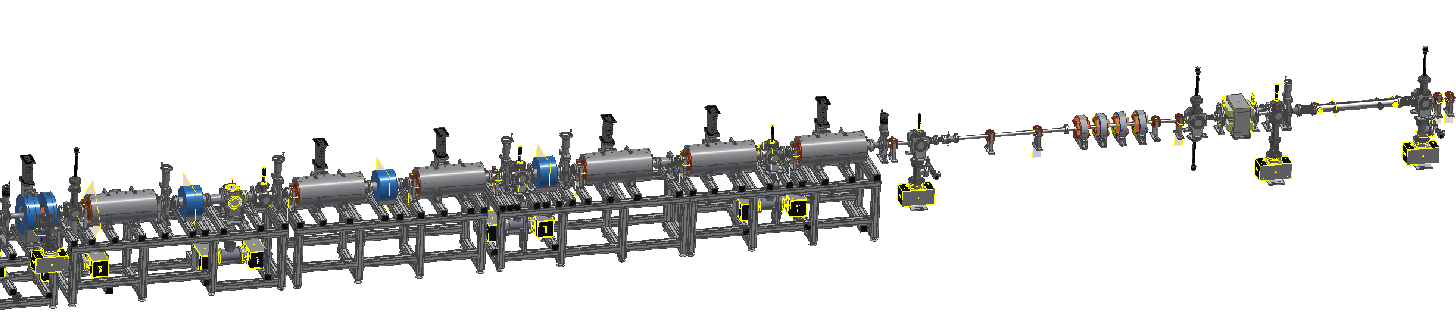
\includegraphics[width=\textwidth]{Report/awa-drawing}};
	\node[fill=white, inner sep=2pt] (txt2) at (0,\gunheight) {\large Gun};
	\node[fill=white, inner sep=2pt] (txt2) at (20,\gunheight) {\large Accelerating Cavities};
	\node[fill=white, inner sep=2pt] (txt2) at (\quadleft,\quadheight) {\large Quadrupoles};
	\draw [blue, ->, line width=1] (\quadleft+\leftarrow,\topofarrows) -- (\quadleft+\leftarrow, \bottomofarrows);
	\node[fill=white, inner sep=2pt] (txt2) at (\kickerleft,20) {\large $s_1$};
	\node[fill=white, inner sep=2pt] (txt2) at (\kickerleft+8,20) {\large $s_2$};
	\node[fill=white, inner sep=2pt] (txt2) at (\kickerleft,\quadheight) {\large Kicker};
	\draw [blue, ->, line width=1] (\kickerleft+\leftarrow-3,\topofarrows) -- (\kickerleft+\leftarrow-3, \bottomofarrows);	
	\draw [black, ->, line width=1] (0,-2) -- (100, -2);
	\node[fill=white, inner sep=2pt] (txt2) at (50,0) {\large Beam Direction};
	\end{tikzpicture}
	\caption{Side view of the high charge linac at the AWA. 
		All hardware in this drawing is currently installed.}
	\label{awa-linac}
	\vspace{-7em}
\end{figure*}

\def \septheight {65}
\def \bottomarrow {57}
\def \kleft {13}
\def \sleft {41.5}
\def \sheight {47}
\def \beam {35}
\begin{figure*}
	\begin{tikzpicture}[every node/.style={anchor=south west,inner sep=0pt},x=1mm, y=1mm,]   
	\node (fig2) at (0,0)
	{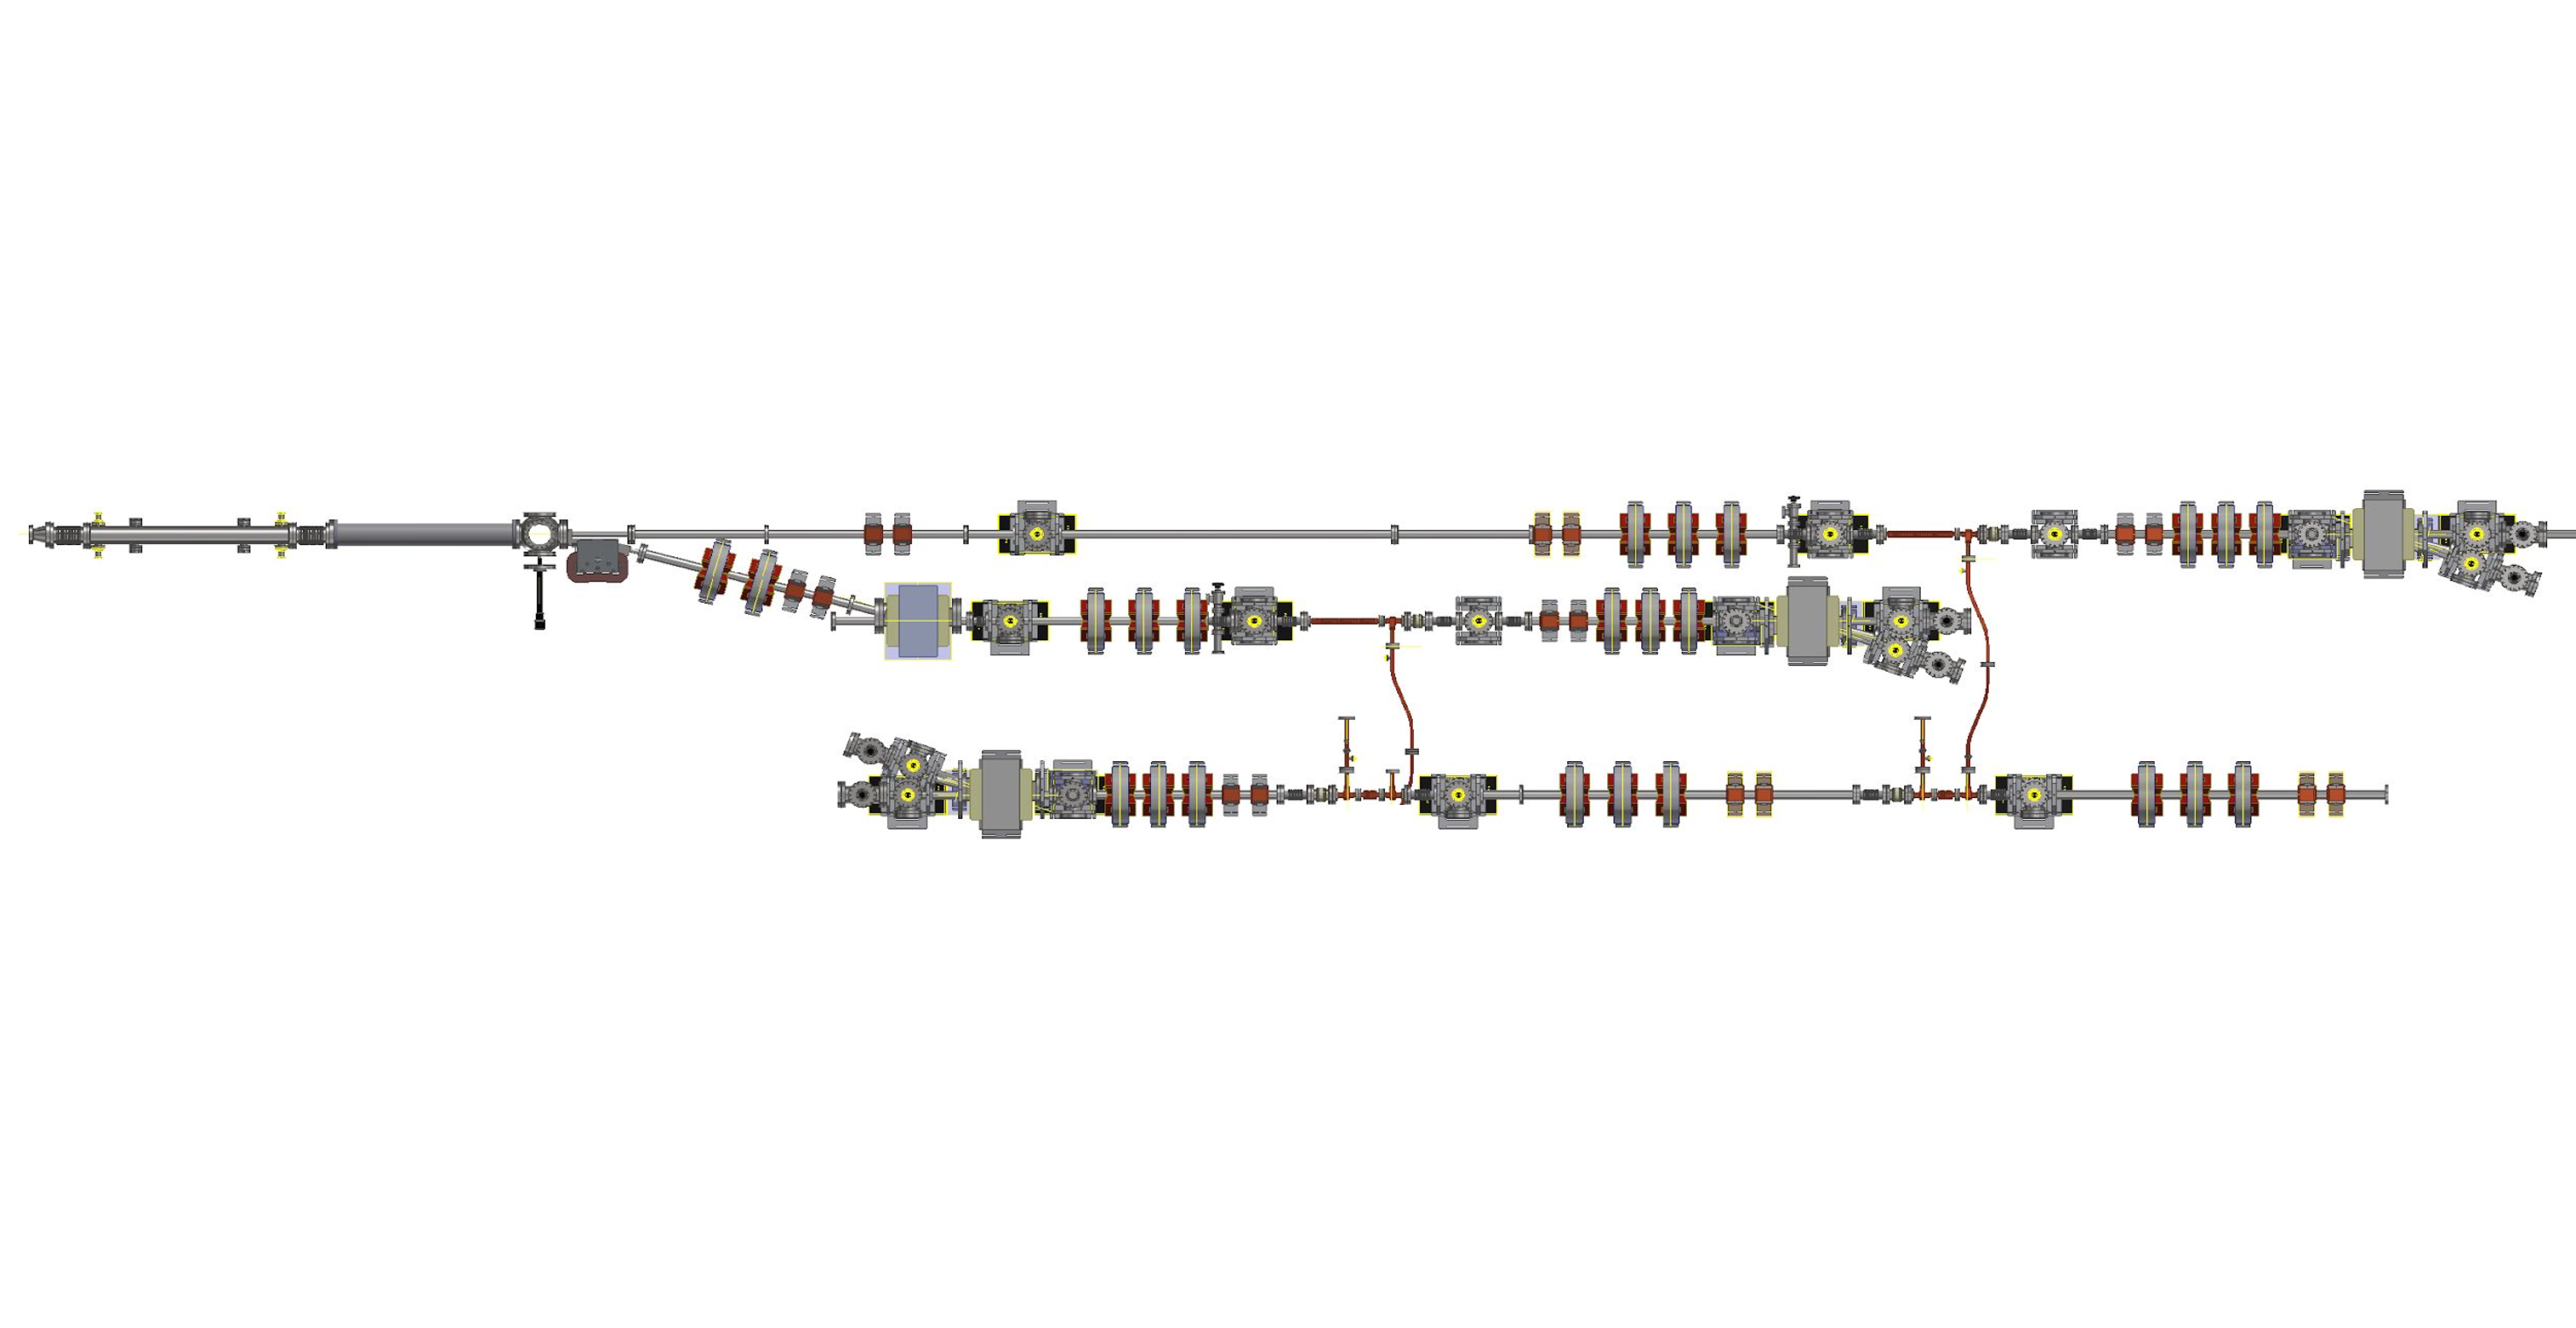
\includegraphics[width=\textwidth]{Report/tba_dogleg}};
	\node[fill=white, inner sep=2pt] (txt2) at (3,\sheight) {\large $s_1$};
	\node[fill=white, inner sep=2pt] (txt2) at (20,\sheight) {\large $s_2$};
	\node[fill=white, inner sep=2pt] (txt2) at (46,45) {\large $s_3$};
	\node[fill=white, inner sep=2pt] (txt2) at (33,\septheight) {\large Septum};
	\draw [blue, ->, line width=1] (\sleft,\septheight) -- (\sleft, \bottomarrow);	
	\node[fill=white, inner sep=2pt] (txt2) at (7,\septheight) {\large Kicker};
	\draw [blue, ->, line width=1] (\kleft,\septheight) -- (\kleft, \bottomarrow);
	\draw [black, ->, line width=1] (0,\beam) -- (100,\beam);
	\node[fill=white, inner sep=2pt] (txt2) at (50,\beam+2) {\large Beam Direction};
	\end{tikzpicture}
	\vspace{-12em}
	\caption{Continuation of the high charge beam line layout at the AWA, top view. 
		This is the proposed two beam acceleration section. 
		Only the kicker in this drawing is installed}
	\label{awa-tba}
\end{figure*}
%
%\vspace{-1em}

In addition to the physics challenges, we chose this model to demonstrate the ability of the framework to tackle large problems.
Six design variables and objectives were used, along with three constraints.
The objectives include transverse and longitudinal beam sizes, 
transverse momentum, and longitudinal energy spread. 
The design variables include the two gun solenoids and 
the first four quadrupoles. 
This problem encompasses high dimensionality 
and nonlinear effects such as space charge. There is no existing information
that accurately predicts where the Pareto fronts will fall. This work is also meaningful in that
it will guide future operations at the AWA.


\subsubsection{Time Step Scan} \label{awa:subsection:test}
Before running a full scale optimization of the problem described in Subsection \ref{awaproblem}, 
a study on time step and number of particles in the simulation model 
was done to reduce the time to simulation while 
maintaining the physics of interest. 
The grid size $16 \times 16 \times 32$ was chosen, 
and parallelized in the x and y directions.
After comparing several options (1,000, 10,000, 20,000, 50,000, 100,000) 
with a small time step, the number of particles was fixed at ten thousand.
Next several time steps were explored, see Table~\ref{timestep}.
The largest steps were too big to resolve the physics needed.
See low fidelity plot in Fig.~\ref{tstep} for $dT=$\num{5E-11} results.  

\begin{table}%[h!]
	\begin{center}
		\caption{Checkmarks (\cmark) indicate desired physics is resolved at that time step. 
			An (\xmark) indicates the time step is too large, and results are nonphysical.}
		\label{timestep}
		\begin{tabular*}{0.48\textwidth}{c @{\extracolsep{\fill}} C c D }
			\hline\noalign{\smallskip}
			Time Step (dT) & Linac & Drift & Quadrupoles \\
			\noalign{\smallskip}\hline\noalign{\smallskip}
			$5 \times10^{-10}$  & \xmark & \xmark & \xmark \\
			$1 \times10^{-10}$  & \xmark & \xmark & \xmark \\
			$5 \times10^{-11}$  & \xmark & \xmark & \xmark \\
			$1 \times10^{-11}$  & \cmark & \cmark & \xmark \\
			$5 \times10^{-12}$  & \cmark & \cmark & \xmark \\
			$1 \times10^{-12}$  & \cmark & \cmark & \cmark \\
			\noalign{\smallskip}\hline
		\end{tabular*}
	\end{center}
\end{table}

In the drifts and linac tanks, $dT=\num{1E-11}$ was sufficient, 
but not acceptable near the quadrupoles. 
For all models, the longitudinal parameters (rms$_s$ and energy) 
are calculated correctly, but we see discrepancies in the transverse 
(rms$_x$ and $\epsilon_x$) for low fidelity results. This discrepancy is 
what led to the decision to adjust the time steps w.r.t. beam line elements. 
In the linac and drift sections $dT=\num{1E-11}$ was used. 
A time step of $dT=\num{1E-12}$ was used near sensitive elements such as the quadrupoles, kicker, and septum. 

The resulting simulations are low fidelity in most places, but closely approximate 
the mid fidelity simulations for metrics of interest, as shown in 
Fig.~\ref{tstep}.  Where we consider mid fidelity as a simulation of the 
beam line using $dT=\num{1E-12}$ everywhere. The
average run time of each simulation with the adjusted time steps was 1.6~minutes.
In comparison, the mid fidelity simulation ran for 18~minutes.
Note, a smaller time step, \num{1E-13}, is always used in the gun where the 
beam is low energy and changing rapidly.
%A summary of the parameters used is listed in Table \ref{fidelity}. 

\begin{figure}%[h]
	\centering
	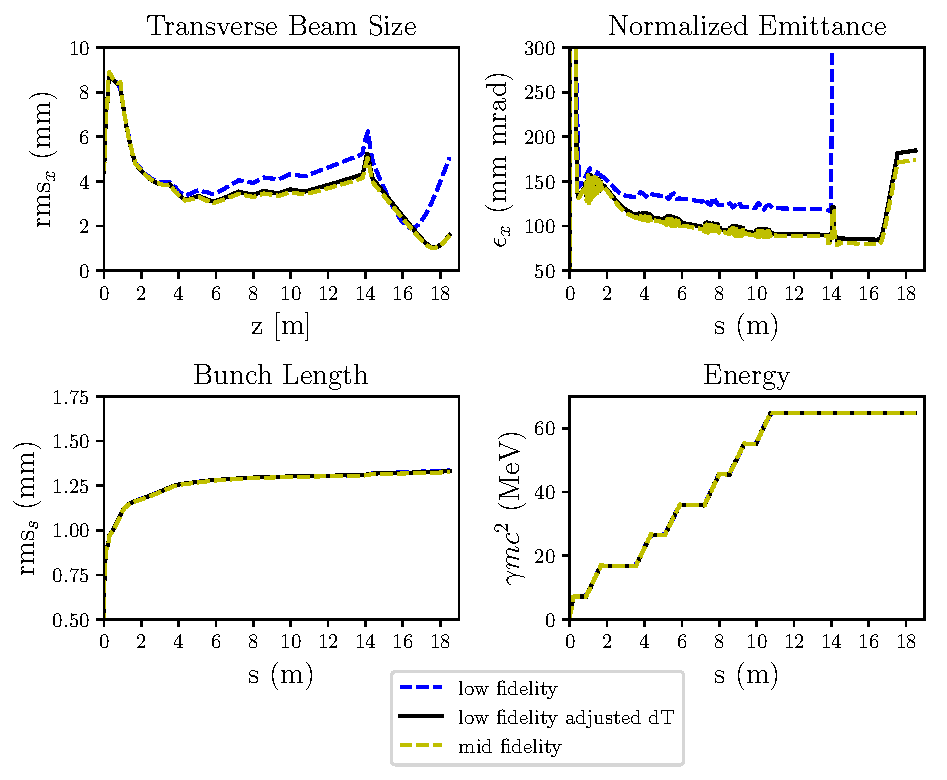
\includegraphics[width=\linewidth]{Report/timestep_comparison}
	\caption{Comparison of different fidelity models (dT stands for time step).}
	\label{tstep}
\end{figure}


\iffalse
\begin{table}%[h!]
	\begin{center}
		\caption{Low and mid fidelity simulation parameters.}
		\label{fidelity}
		\begin{tabular*}{0.48\textwidth}{l @{\extracolsep{\fill}} C c D }
			\hline\noalign{\smallskip}
			& Number of particles & dT (seconds) & Time to simulation (minutes)\\
			\noalign{\smallskip}\hline\noalign{\smallskip}
			low fidelity  			&  10,000   & $5 \times10^{-11}$  &  2.6 \\
			adjusted low fidelity  	&  10,000   & $2 \times 10^{-12}$, $1 \times 10^{-11}$ & 1.6 \\
			mid fidelity 			&  100,000  & $1 \times 10^{-12}$ &  18\\
			\noalign{\smallskip}\hline
		\end{tabular*}
	\end{center}
\end{table}
\fi 

\subsubsection{Hyper parameter Scan}
While the optimization problem and goals were well defined (Subsection \ref{awaproblem}), 
it was not clear what the best hyper parameters for the NSGA-II would be.
These parameters include gene mutation probability, mutation probability, 
recombination probability, number of individuals, 
and number of generations to complete. 
Given the beam line in Fig.~\ref{awa-linac},
four small optimization experiments were done with varying NSGA-II parameters. 
Similar to the time step scan, 
the goal of this exercise was to determine which set of optimization
parameters strongly influence the results, 
and whether there was a time to solution difference.
From here on, we will reference each experiment as ex-1, ex-2, ex-3, and ex-4
as shown in Table \ref{extable}. 
\begin{table}%[h!]
	\begin{center}
		\caption{Input Parameters for initial twenty four hour AWA optimization experiments. 
			The gene mutation probability was equal to the mutation probability (not shown) in all four experiments. 
			The max number of individuals per generation was~80.}
		\label{extable}
		\begin{tabular*}{0.48\textwidth}{l @{\extracolsep{\fill}} C C D }
			\hline\noalign{\smallskip}
			& Gene Mutation Probability & Recombination Probibility & Number of completed generations \\
			\noalign{\smallskip}\hline\noalign{\smallskip}
			ex-1 &  0.1  & 0.9  &  96 \\
			ex-2 &  0.3  & 0.7  &  81 \\
			ex-3 &  0.8  & 0.2  &  53 \\
			ex-4 &  0.01 & 0.09 &  95 \\
			\noalign{\smallskip}\hline
		\end{tabular*}
	\end{center}
\end{table}


The maximum number of individuals per generation was fixed at 80, 
Each experiment was allowed to run for twenty four hours, with 
a maximum generation limit of 100. 
We reduced the six objectives to four, 
and shortened the simulation time by moving the objectives further 
upstream to $s_1$ and $s_2$.
The objectives include: $\varepsilon_{x}\left(s = s_1\right)\text{, } \varepsilon_{x}\left(s = s_2\right)\text{, } \text{rms}_{s}\left(s = s_1\right)\text{, and }  \text{rms}_{s}\left(s = s_2\right)$. 
\lsnote{You could define $\varepsilon_{x1}$ to be $\varepsilon_{x} (s=s1)$ and similarly in the table and then use going forward to simplify notation}
The OPAL input file for ex-3 is given as an example to show how optimization and design variables are defined:
%

%\vspace{0.2cm}
\begin{Verbatim}[fontsize=\scriptsize]
OPTION, ECHO=FALSE;
OPTION, INFO=TRUE;

TITLE, STRING="ANL Optimisation";

dv0: DVAR, VARIABLE="IBF",    LOWERBOUND=200.0, UPPERBOUND=500.0;
dv1: DVAR, VARIABLE="IM",     LOWERBOUND=170.0, UPPERBOUND=260.0;
dv2: DVAR, VARIABLE="GPHASE", LOWERBOUND=-30.0, UPPERBOUND=0.0;
dv3: DVAR, VARIABLE="FWHM",   LOWERBOUND=1.5,   UPPERBOUND=10.0;

// Quad values
dv4: DVAR, VARIABLE="KQ1", LOWERBOUND=-8.0, UPPERBOUND=8.0;
dv5: DVAR, VARIABLE="KQ2", LOWERBOUND=-8.0, UPPERBOUND=8.0;
dv6: DVAR, VARIABLE="KQ3", LOWERBOUND=-8.0, UPPERBOUND=8.0;
dv7: DVAR, VARIABLE="KQ4", LOWERBOUND=-8.0, UPPERBOUND=8.0;

rmss1:  OBJECTIVE,EXPR="fabs(statVariableAt('rms_s',16.5))";
emitx1: OBJECTIVE,EXPR="fabs(statVariableAt('emit_x',16.5))";

rmss2:  OBJECTIVE,EXPR="fabs(statVariableAt('rms_s',18.5))";
emitx2: OBJECTIVE,EXPR="fabs(statVariableAt('emit_x',18.5))";

c1: CONSTRAINT, EXPR="fabs(statVariableAt('rms_x',16.5))<1.0e-1";
c2: CONSTRAINT, EXPR="fabs(statVariableAt('rms_y',16.5))<1.0e-1";


OPTIMIZE, INPUT="tmpl/optLinac_40nC.tmpl",
OUTPUT="optLinac_40nC",
OUTDIR="results",
OBJECTIVES = {rmss1, emitx1, rmss2, emitx2},
DVARS = {dv0, dv1, dv2, dv3, dv4, dv5, dv6, dv7},
CONSTRAINTS = {c1, c2},
INITIALPOPULATION=80,
MAXGENERATIONS=100,
NUM_MASTERS=1,
NUM_COWORKERS=8,
SIMTMPDIR="tmp",
TEMPLATEDIR="tmpl",
\end{Verbatim}
%\vspace{0.2cm}

After collection of the data for all four experiments, several metrics
were compared, including number of generations completed in twenty four hours and
Pareto fronts at $s_1$ and $s_2$.
From Table \ref{extable}, we clearly see ex-3 is significantly 
slower, as it evaluated only 53 generations compared to the max 
experiment, ex-1 at 96 generations.
Perhaps this trade off would be acceptable if the Pareto front was significantly 
improved, but from Fig. \ref{expareto}, we can see this is not the case.
Similar arguments can be made for ex-2, which evaluated about 15 less generations
with no clear benefit in either Pareto front.
The Pareto fronts at $s_1$, are nearly identical. We could expect
this trend would continue given more time. 
When looking at the Pareto front at $s_2$, only ex-4 has a slight 
edge over the others.
With ex-2 and ex-3 eliminated due to evaluation time, 
and a slightly better Pareto front at $s_2$ for ex-4, the hyper parameters in ex-4 were chosen as the default values for subsequent runs.


\begin{figure}
	\centering
	\begin{minipage}{0.49\textwidth}
		\centering
		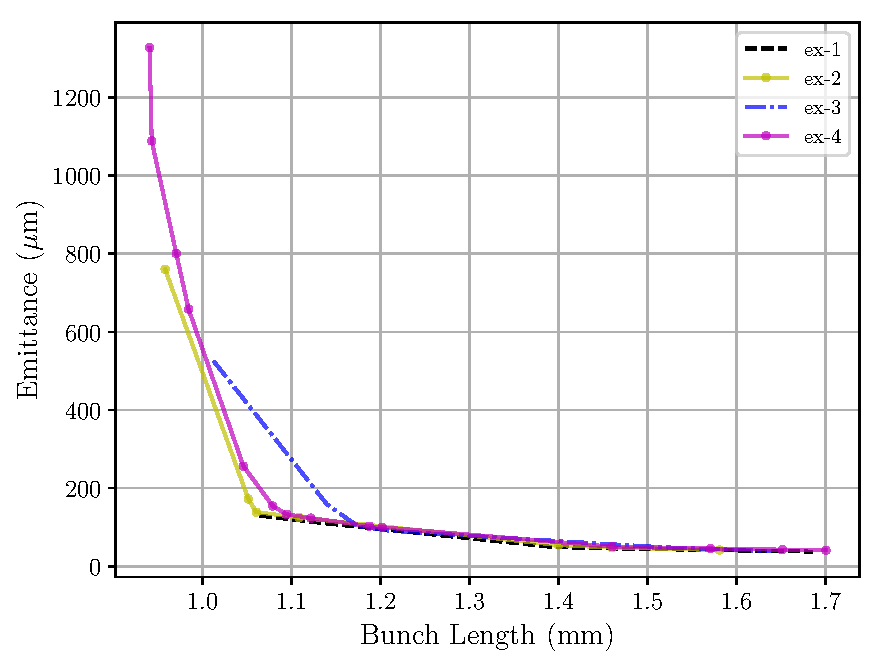
\includegraphics[width=\textwidth]{Report/ex-pareto1}
		(a) Pareto fronts for ex-1 through ex-4 at $s_1$.
		%\caption{(a) Pareto fronts at $s_1$.}
		%\label{expareto1}
		\vspace{2em}
	\end{minipage}
	\begin{minipage}{0.49\textwidth}
		\centering
		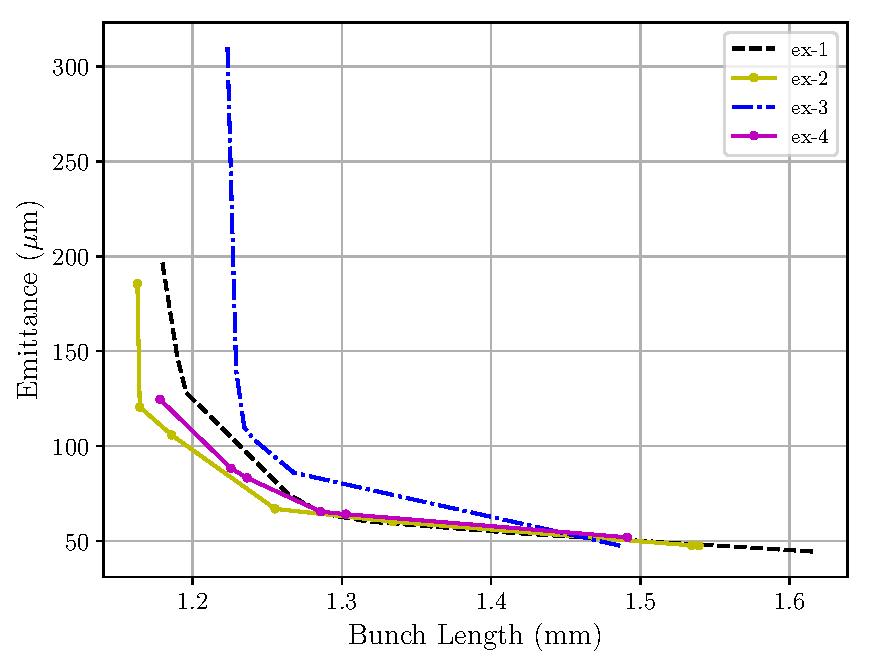
\includegraphics[width=\textwidth]{Report/ex-pareto2}
		(b) Pareto fronts for ex-1 through ex-4 at $s_2$.
		%\caption{(b) Pareto fronts at $s_2$.}
		%\label{expareto2}
	\end{minipage}
	\caption{Comparison of Pareto fronts for initial optimization experiments, ex-1 through ex-4.}
	\label{expareto}
\end{figure}





\subsubsection{TBA Optimization Problem}
With computational and hyper parameters set, 
the full optimization problem of interest is explored.
The objectives (beam sizes and energy spread) are calculated at 
$s_3=19.4$~m. See Fig.~\ref{awa-tba} for location of $s_3$ w.r.t. other 
beam line elements. 
Given the longitudinal location of $s_3$ (unless otherwise noted), 
we define the objectives and input parameters as:
\begin{align}
\text{min}  \quad & \text{rms}_{x}, \quad \text{rms}_{y} \label{eq:awa:p1}\\
& \text{rms}_{px}, \quad \text{rms}_{py}, \label{eq:awa:p2}\\
& \text{rms}_{s}, \quad dE \label{eq:awa:p4} \\
\text{constraints} \quad & rms_x < 0.1 \, [m] |_{s=s_1}\label{eq:awa:c1}\\
\quad & rms_y < 0.1 [m] |_{s=s_1}\, \label{eq:awa:c2}\\
\quad & |rms_y - rms_x | < 0.005 \, [m] |_{s=s_1}\label{eq:awa:c3}\\
\text{subject to} \quad & q = 40 \left[\text{nC}\right] \label{eq:awa:firstconstr}\\
\quad & \text{Volt}_{\text{Gun}} = 64\left[\text{MV/m}\right] \label{eq:awa:lastconstr}\\
\quad & \text{Volt}_{\text{Linac}} = 24 \, \text{or} \, 25\left[\text{MV/m}\right] \\
\quad & R_x = R_y = 9 \left[\text{mm}\right] \label{eq:awa:firstdvar}\\
\quad & \phi_{\text{gun}} =-20^\circ \label{eq:awa:gphidvar}\\
\quad & \phi_{\text{linac}} =-20^\circ \label{eq:awa:lastdvar}
\end{align}



The first four objectives, Eqs. (\ref{eq:awa:p1}) to (\ref{eq:awa:p2}),
minimize the transverse ($rms_{x,y}$) beam size and transverse momentum ($rms_{px,py}$)
at the location of interest in the beam line ($s_3$).
%Where $s_3$ is the longitudinal entrance of the fifth quadrupole. 
Minimizing the beam size at this location is essential to 
to preventing loss of particles by scraping; 
which ensures better transmission through the wakefield structures downstream. 
Less divergence in the beam (lower transverse momentum) 
reduces growth of transverse beam size after the focal point (min beam size).
This reduces halo by ensuring the beam is not over focused through a hard waist.
The momentum is also critical to preventing large growth during transport in bending elements. 
All of these factors help with transmission downstream. 

The next two objectives in Eq. (\ref{eq:awa:p4}) minimize the 
longitudinal beam size ($rms_s$), and energy spread (dE) at location $s_3$.
This helps reduce longitudinal beam size growth in bending elements.
A small bunch length ($rms_s$) is also critical to the goals of 
TBA experiments. The power generated in the wakefield structures 
designed for TBA is related to the bunch length \cite{JING201872}.
\nrnote{need better source for this info} 
i.e. smaller bunch lengths result in larger wakefields and higher power generation.
 
  

Eqs.~\ref{eq:awa:c1} to \ref{eq:awa:c3} 
define three constraints used to guide the algorithm.
The bounding values may seem large, but this is done to avoid over constraining the 
problem in early generations. When the constraints were set tighter, 
optimization runs did not reach the second generation within a 48 hour time limit. 
In other words, enough satisfactory points were not produced to fill a complete generation in 48 hours. 
By leaving the value large, a sufficient number of simulations finish
and subsequent generations are reached in a timely manner. 
As multiple generations, the objectives continue to improve.

The difference constraint, Eq.~\ref{eq:awa:c3}, is used to favor nearly round beams.
This prevents one dimension from becoming disproportionately large compared to the other.
At the AWA, there is some room in the beam pipe to allow the y dimension to grow, but round beams 
are preferred for easier data analysis.

Equations (\ref{eq:awa:firstconstr}) to
(\ref{eq:awa:lastdvar}) define the charge, gun voltage, linac voltages, 
laser radius, gun phase, and linac cavity phases (in that order). 
These are parameters in the simulation 
that must be defined, but do not vary during the optimization.
%\vspace{-1em}
As introduced in Section \ref{ferrario}, we define the AWA optimization 
design variables, objectives, and constraints in the OPAL input file as shown in
the following code: %equations (\ref{eq:awa:p1}) to (\ref{eq:awa:lastdvar}). 
%\vspace{0.2cm}
\begin{Verbatim}[fontsize=\scriptsize]

// Gun variables 
dv0: DVAR, VARIABLE="IBF",    LOWERBOUND=300.0, UPPERBOUND=500.0;
dv1: DVAR, VARIABLE="IM",     LOWERBOUND=180.0, UPPERBOUND=280.0;

// Quad variables 
dv4: DVAR, VARIABLE="KQ1", LOWERBOUND=-8.0, UPPERBOUND=8.0;
dv5: DVAR, VARIABLE="KQ2", LOWERBOUND=-8.0, UPPERBOUND=8.0;
dv6: DVAR, VARIABLE="KQ3", LOWERBOUND=-8.0, UPPERBOUND=8.0;
dv7: DVAR, VARIABLE="KQ4", LOWERBOUND=-8.0, UPPERBOUND=8.0;

//Objectives
de3: OBJECTIVE,EXPR="fabs(statVariableAt('dE',19.4))";
rmss3: OBJECTIVE,EXPR="fabs(statVariableAt('rms_s',19.4))";
rmsx3: OBJECTIVE,EXPR="fabs(statVariableAt('rms_x',19.4))";
rmsy3: OBJECTIVE,EXPR="fabs(statVariableAt('rms_y',19.4))";
rmspx3: OBJECTIVE,EXPR="fabs(statVariableAt('rms_px',19.4))";
rmspy3: OBJECTIVE,EXPR="fabs(statVariableAt('rms_py',19.4))";

//Kicker apeture
c1: CONSTRAINT, EXPR="fabs(statVariableAt('rms_x',16.5))<0.1";
c2: CONSTRAINT, EXPR="fabs(statVariableAt('rms_y',16.5))<0.1";
c3: CONSTRAINT, EXPR="fabs(statVariableAt('rms_y',16.5)
			-statVariableAt('rms_x',16.5))<0.005";

OPTIMIZE, INPUT="tmpl/optLinac-40nC.tmpl",
OUTPUT="optLinac-40nC",
OUTDIR="results",
OBJECTIVES = {rmss3, rmsx3, rmsy3, rmspx3, rmspy3, de3},
DVARS = {dv0, dv1, dv4, dv5, dv6, dv7},
CONSTRAINTS = {c1, c2, c3},
INITIALPOPULATION=656,
MAXGENERATIONS=200,
NUM_MASTERS=1,
NUM_COWORKERS=8,
SIMTMPDIR="tmp",
TEMPLATEDIR="tmpl",
FIELDMAPDIR="fieldmaps",
NUM_IND_GEN=328,
GENE_MUTATION_PROBABILITY=0.01,
MUTATION_PROBABILITY=0.01,
RECOMBINATION_PROBABILITY=0.09;
QUIT;
\end{Verbatim}
\vspace{0.2cm}

Design variables include the currents in two gun solenoids (IBF and IM), 
and four quadrupole strengths (KQ1-KQ2). The objectives include
beam size (transverse and longitudinal), transverse momentum, and energy spread as
defined in Eqs. (\ref{eq:awa:p1}) to (\ref{eq:awa:p4}). 
The location at the entrance of the kicker is $s_1=16.45$~meters, 
and the location of interest for objectives is $s_3=19.4$~meters. 


\subsubsection{AWA Optimization Results}
All simulations for this experiment were carried out on Bebop a
high performance computing (HPC)
cluster provided by the Laboratory Computing Resource Center (LCRC)
at Argonne National Laboratory (ANL). We used Intel Knights Landing 
(KNL) processors at 1.3 GHz with 128 GB of memory 
and 64 cores per node. There are 352 compute nodes available on 
Bebop, with a total of 22,528 cores. All jobs were run and compared 
on 8 cores each, which allowed 8 jobs per node on the KNLs.
This in combination with the number of nodes available 
allows for very large optimization jobs, like the AWA case.
Typical runs for this paper used 41 nodes, which corresponds to 2624 KNL cores 
and a generation size of 328 individuals.


With the time steps and hyper parameters set by the work in Section \ref{awa:subsection:test}, 
the full optimization problem described in \ref{awaproblem} was run for 200 generations.
The initial number of individuals was fixed at 656, 
and the minimum number individuals in later generations was fixed at 328. 
These numbers were in part based on the architecture of the KNL's. 
Since each simulation takes 8 cores, and there are 64 cores per KNL node, 
we wanted a large population size that would fit evenly on these resources. 

Again, the location of optimization is $s_3=19.4$ [m]. 
This is the entrance to the fifth quad in the beam line. 
This location is where the beam should be captured and focused through subsequent elements.
After collection of the data, Pareto fronts comparing the objectives were plotted, 
see Figs.~\ref{fig:pareto1} and \ref{fig:pareto2}.

\begin{figure}
	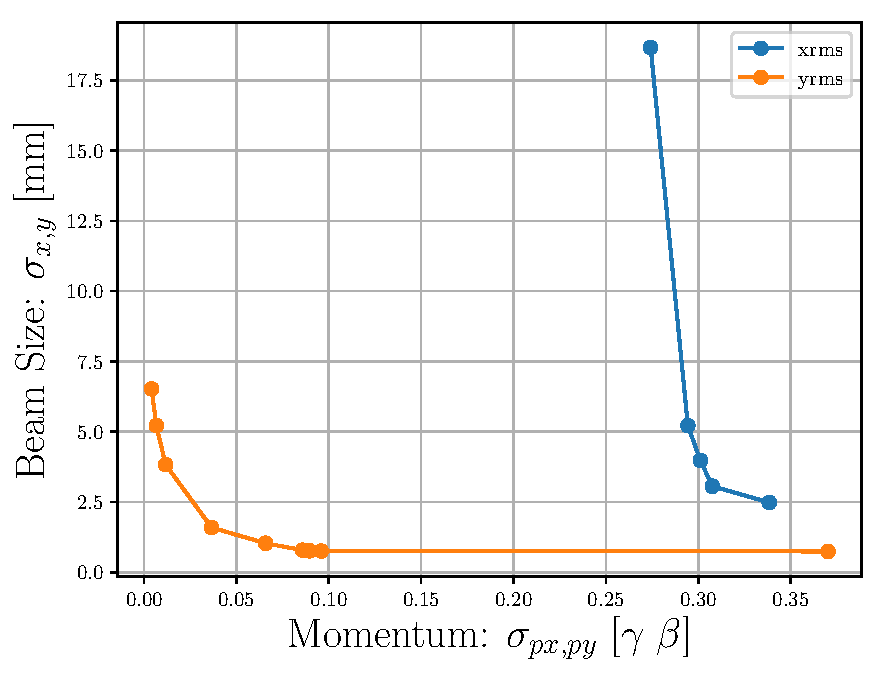
\includegraphics[width=0.5\textwidth]{../pareto_stat_plots/xy_vs_pxy_pareto_front_quads_before_Q5}
	\caption{Pareto front comparing transverse beam sizes ($\sigma_{x,y}$) and transverse momentum ($\sigma_{px,py}$).}
	\label{fig:pareto1}
\end{figure}

 
\begin{figure}
	\centering
	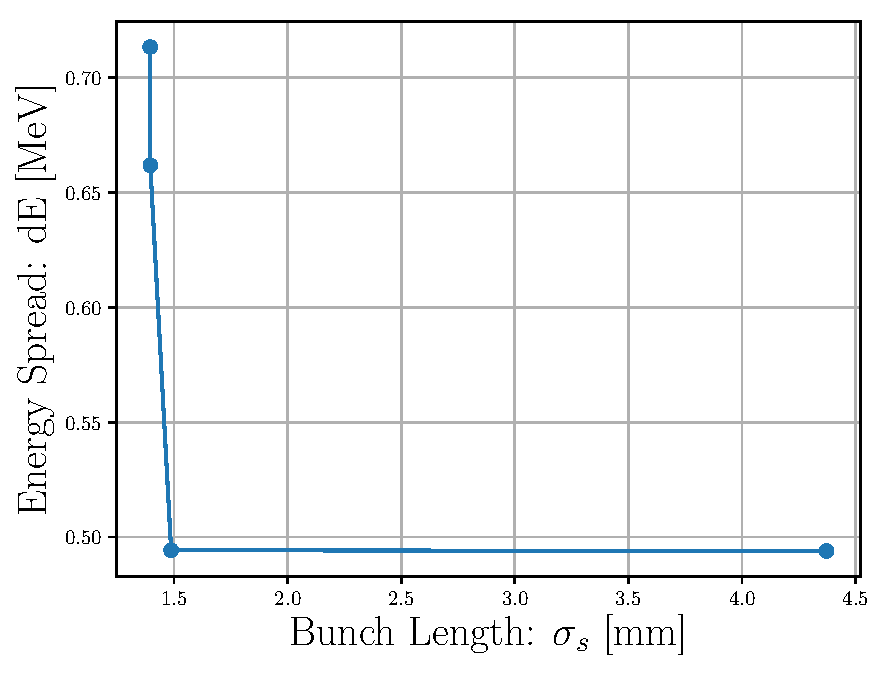
\includegraphics[width=0.48\textwidth]{../pareto_stat_plots/dE_vs_zrms_pareto_front_quads_before_Q5_zoomout}%
	\llap{\raisebox{1.9cm}{%  move next graphics to top right corner
			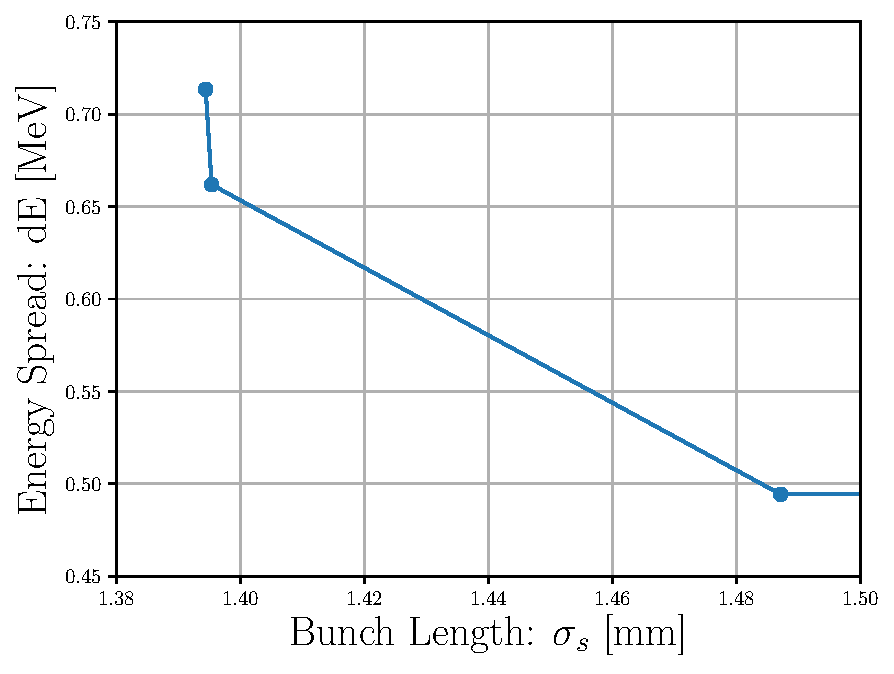
\includegraphics[height=4.5cm]{../pareto_stat_plots/dE_vs_zrms_pareto_front_quads_before_Q5}%
	}}
	\caption{Pareto front comparing energy spread (dE) and bunch length ($\sigma_z$). \nrnote{add tikz arrows to point to left side of curve?}}
	\label{fig:pareto2}
\end{figure}  


As expected, the x dimension is impacted by the bending elements, and unable to reach 
the small beam sizes seen in the y dimension. This suggest objectives in the x 
dimension will drive design variable choices used in operations. 
However, it is still necessary to 
include the y dimension in optimization. Early optimization tests showed the y dimension 
can easily grow out of control if not included in the objectives.
Those results are not shown here due to the unfeasible solutions they resulted in
(i.e. $rms_y$ larger than the beam pipe).
In the case of bunch length, there are not many options to choose from.
Ignoring the extreme value on the right, Fig.~\ref{fig:pareto2} shows the 
range of optimal bunch lengths fall between 1.39 and 1.5 mm.

With these observations in mind, several beam parameters corresponding to
options on Pareto Front in Fig.~\ref{fig:pareto1} were plotted and compared. 
A select result is shown in Fig.~\ref{fig:stat}. 
The maximum beam sizes are well below the beam pipe aperture limits as shown in Fig.~\ref{fig:stat} (b).
The solution is nearly round, which will increase changes of keeping the beam nearly round
as it travels to the last triplet in Fig.~\ref{awa-tba}.
Overall this solution is satisfactory, and meets all requirements at the AWA.


\begin{figure}
	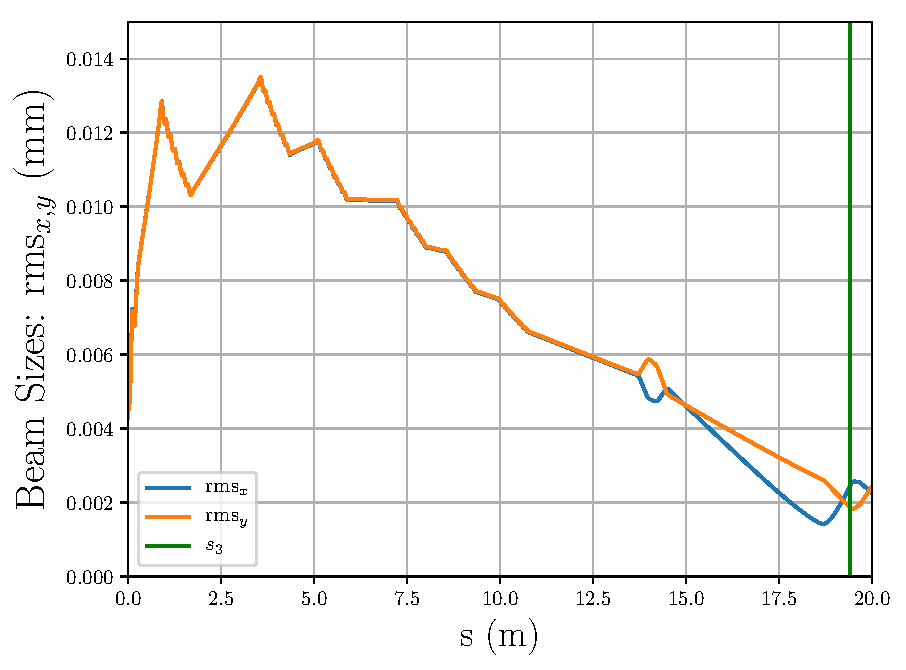
\includegraphics[width=0.48\textwidth]{../pareto_stat_plots/xyrms-zrms_newobj}\\
	\vspace{2em}
	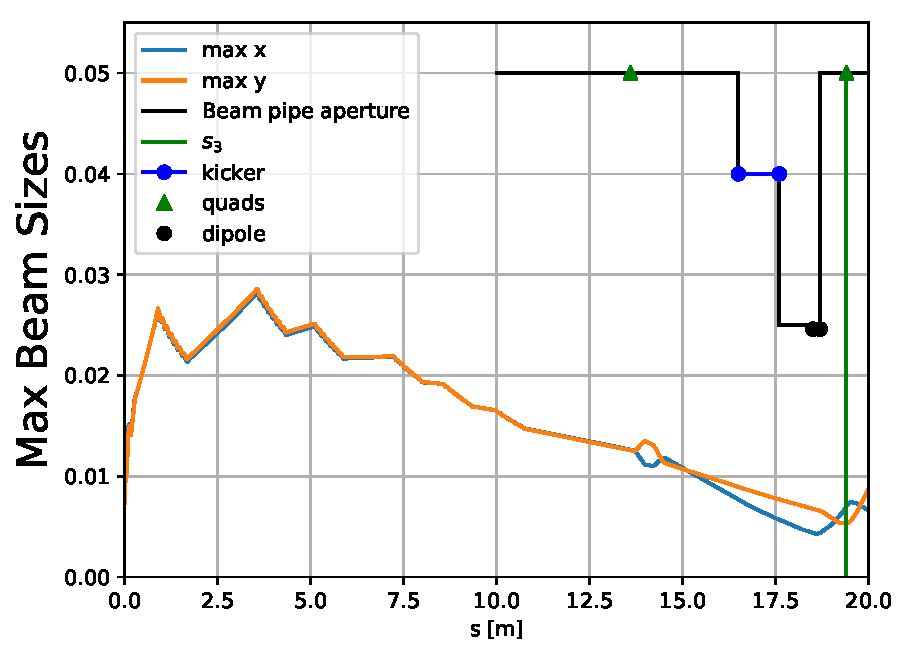
\includegraphics[width=0.48\textwidth]{../pareto_stat_plots/xy-max-min-zrms_newobj}
	\caption{Optimized beam sizes along high charge beam line.}
	\label{fig:stat}
\end{figure}








